\documentclass{standalone}
\usepackage{tikz}
\usepackage{pgfplots}
\pgfplotsset{compat=1.17}

\begin{document}

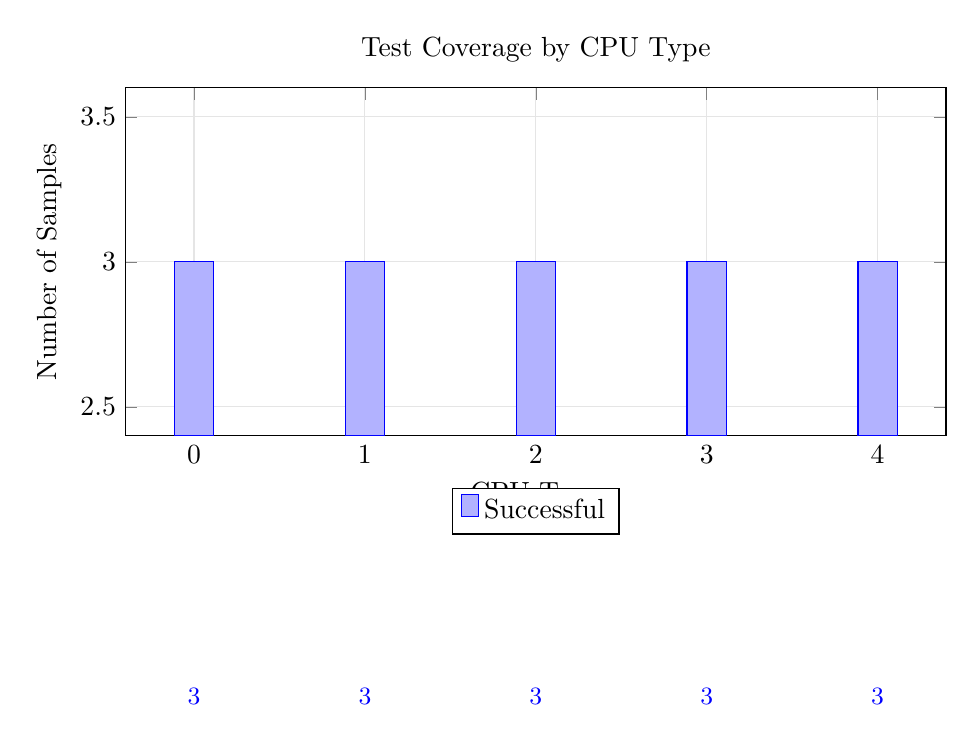
\begin{tikzpicture}
\begin{axis}[
    title={Test Coverage by CPU Type},
    xlabel={CPU Type},
    ylabel={Number of Samples},
    ybar stacked,
    bar width=0.5cm,
    width=12cm,
    height=6cm,
    legend style={at={(0.5,-0.15)}, anchor=north, legend columns=-1},
    xtick=data,
    grid=major,
    grid style={gray!20},
    nodes near coords,
    nodes near coords style={font=\small}
]

\addplot coordinates {
    (0, 3)
    (1, 3)
    (2, 3)
    (3, 3)
    (4, 3)

};
\addlegendentry{Successful}


\end{axis}
\end{tikzpicture}

\end{document}